\section{Variable-Length Encoding Methods}
\label{sec:encoding}

\begin{figure}
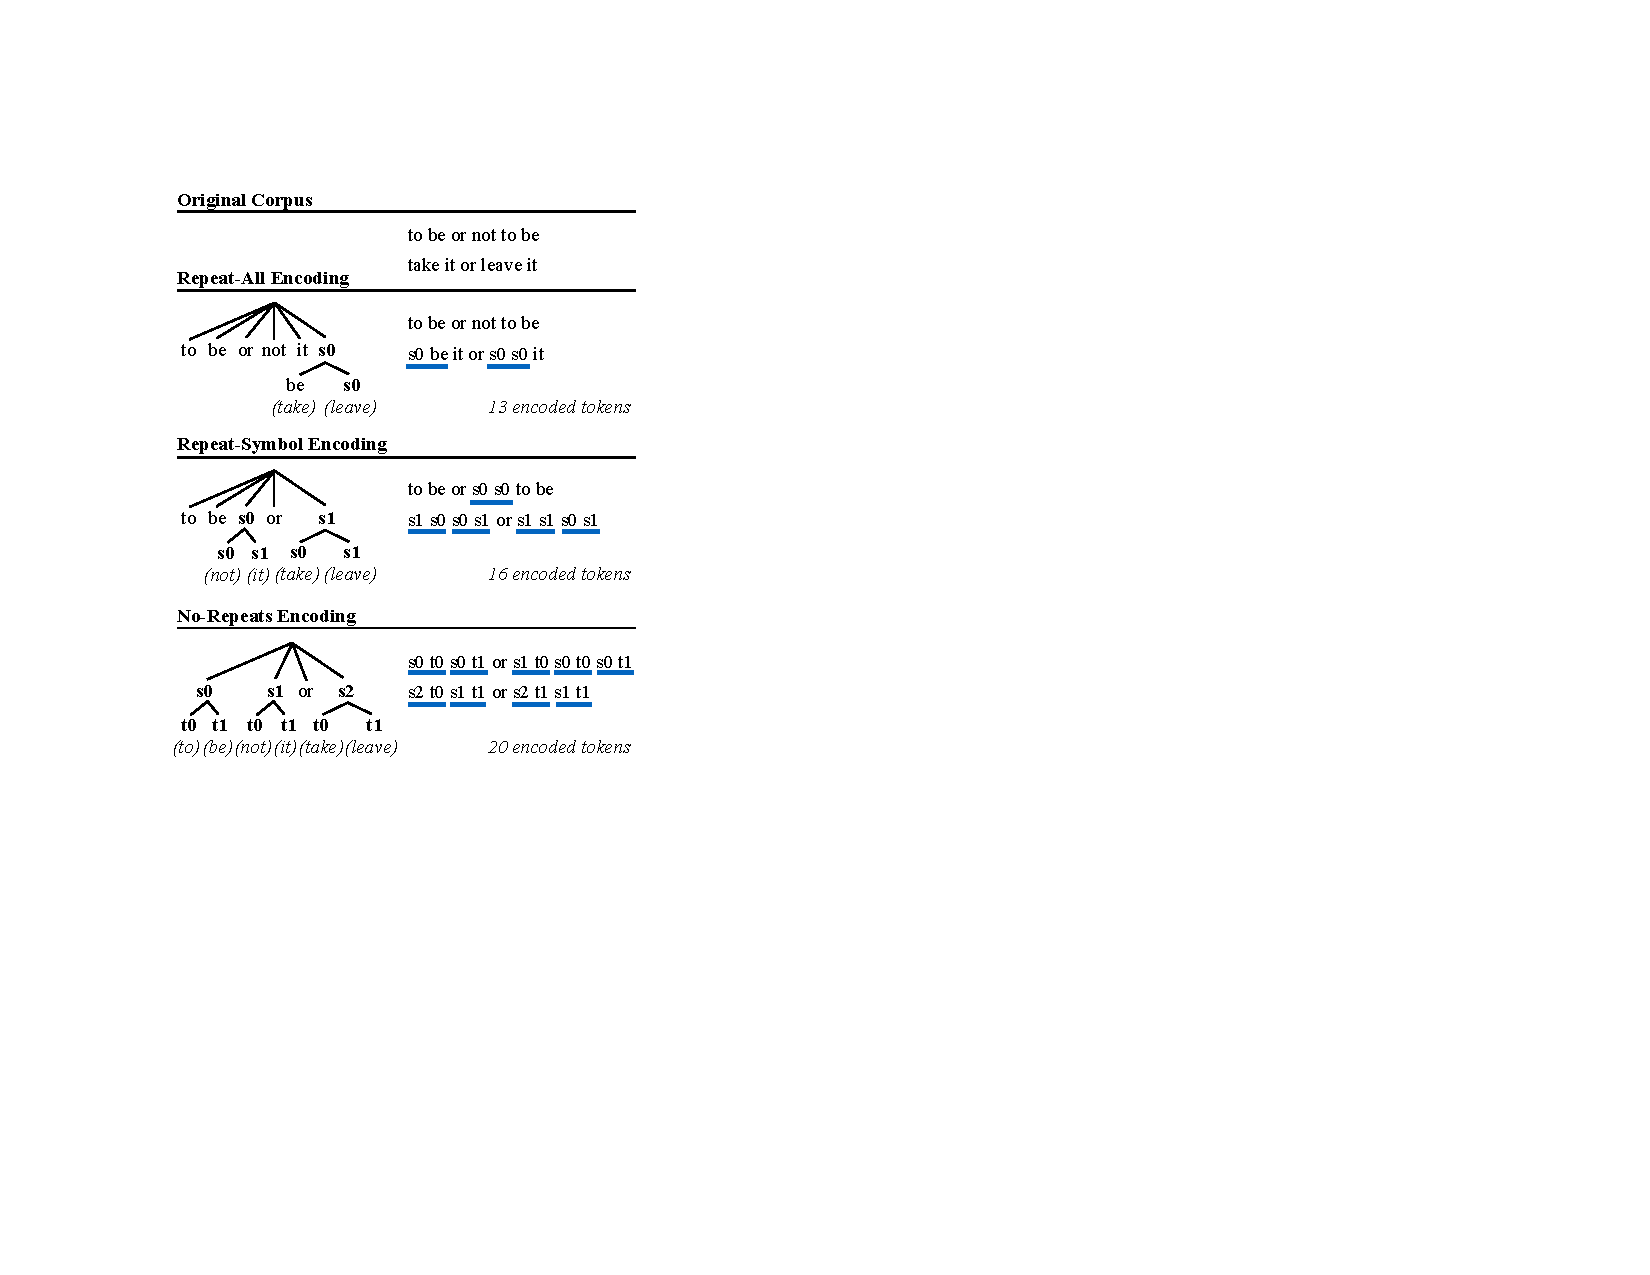
\includegraphics{examples.pdf}
\caption{Our three encoding schemes are applied to a two sentence toy corpus
for which each word type appears one or two times, and the total vocabulary
size $V$ is 7. An optimal encoding tree under each scheme is shown for an
encoded vocabulary size $W$ of 6. As stricter constraints are imposed on the
encoding, the encoded corpus length increases and the number of elements of $V$
that can be represented using a single symbol decreases.
\label{fig:examples}
\end{figure}

We consider three different encoding schemes that are based on Huffman codes.
The encoding for a toy corpus under each scheme is depicted in
Figure~\ref{fig:examples}. While a Huffman code achieves the shortest possible
encoded length using a fixed vocabulary size $W$, symbols are often shared
between both common and rare words. Therefore, a Huffman code may not be
optimal for the task of machine translation using a neural network model. The
variants we consider prevent various forms of symbol sharing.

\subsection{Encoding Schemes}

The first scheme is a standard Huffman code. To construct the encoded
vocabulary $W$, we use

We describe three different invertible encoding schemes. Each one
applies the identity transformation to the words with highest frequency.
It is beneficial to use different encoding schemes because changing the number of
new symbols introduced provides insight into the interaction between number of words
that encode to themselves and the system's ability to learn translations of the encoded words.
We distinguish these highest frequency words by referring to them
as ``common,'' and we call the other words ``rare.''\\

The first encoding scheme, named
``Repeat-All,'' encodes every rare word as two words: a special symbol
of the form ``sXXXX,'' where the X are digits from 0 to 9, followed by any
already-occurring symbol (either a common word or a symbol ``sXXXX'').
 For example, suppose our entire corpus is the sentence ``to be or not to be''
with a common word size of 2. The following diagram shows a possible encoding
tree under the Repeat-All scheme (TODO: add labels to branches and follow style guidelines):

\Tree[. [to ]
        [be ]
        [.s24 [be ] [s27 ]]]

Then, the sentence would be encoded as ``to be s24 be s24 s27 to be.''\\

The second encoding scheme, ``Repeat-Symbol,'' encodes rare words in the
form ``sXXXX sXXXX,'' where as before the X are digits from 0 to 9. Under
this encoding scheme, here is a possible tree for the vocabulary in the
example sentence:

\Tree[. [to ]
        [be ]
        [.s24 [s57 ] [s87 ]]]

Then, the sentence would be encoded as ``to be s24 s57 s24 s87 to be.''\\

Our final encoding scheme, ``No-Repeats,'' encodes rare words in the
form ``sXXXX tXXXX,'' where again the X are digits from 0 to 9. We note that
at the expense of increasing the number of new symbols we introduce into the
vocabulary, the translation system has a better opportunity to learn the
rare word encodings. Here is a possible tree corresponding to the example
sentence:

\Tree[. [to ]
        [be ]
        [.s24 [t57 ] [t87 ]]]

Then, the sentence would be encoded as ``to be s24 t57 s24 t87 to be.''

\subsection{Symbol Counts}
To maximize performance, it is critical to set the number of common words (which
transform to themselves) as high as possible while satisfying the desired total vocabulary size,
counting all the newly introduced symbols. In this section, we algebraically derive
this optimal number of common words for each encoding scheme. We define the following:\\\\
$W$: Number of common words -- first-level terminal nodes in the encoding tree.\\
$V$: Size of the original vocabulary.\\
$K$: Size of the transformed vocabulary (number of words in the encoded text).\\

We are interested in solving for $W$.\\

\textbf{Repeat-All}\\
We would like to encode the $V - W$ rare words, using only $K - W$ new symbols. To do so,
for each new symbol (non-terminal node in our encoding tree), we have all $K$ symbols under
it in that branch. Therefore, we find $$\max_{W} V - W \leq (K - W)K$$
TODO: explain why 2 level tree.\\

\textbf{Repeat-Symbol}\\
Out of the $V - W$ rare words, we would like to pack them into a complete tree so that
they may be encoded using our remaining $K - W$ symbols. Thus, we have $$\max_{W} \sqrt{V - W} \leq K - W$$

\textbf{No-Repeats}\\
We introduce more variables: $S$, the number of non-terminal nodes in the encoding tree (symbols
of the form sXXXX) and $T$, the number of second-level terminal nodes (symbols of the form tXXXX).
As in the Repeat-Symbol derivation, we desire to pack $V - W$ into a complete tree where we
may use $S$ symbols: $\sqrt{V - W} = S$. To maximize $W$, we set $S = T$, so that the number of sXXXX symbols and tXXXX
symbols are the same. Because $S + T + W = K$, we have that $2S + W = K$. Simplifying, we obtain
$$\max_{W} \sqrt{V - W} \leq \dfrac{K - W}{2}$$
